%
% 2d_basisfkt.tex
%
% (c) 2024 Flurin Brechbühler
%
\begin{figure}
    \centering
    \subfloat[In dreieckige Elemente unterteilter zweidimensionaler Definitionsbereich mit nummerierten Knoten \cite{fem:diskretisieren}.]
        {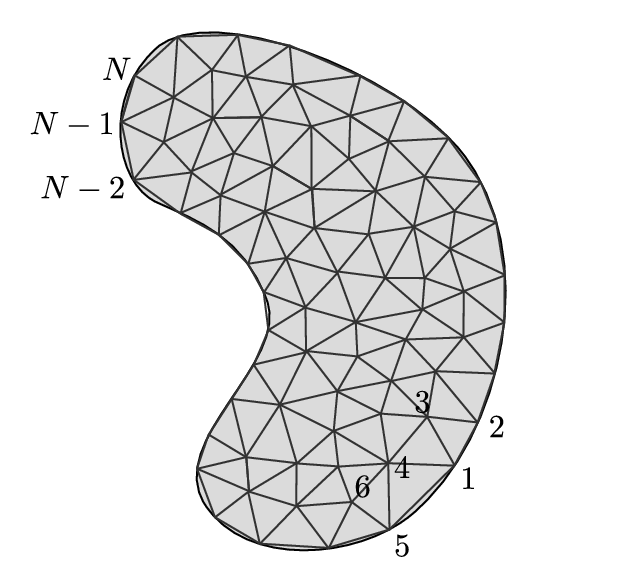
\includegraphics[width = 0.41\textwidth]{papers/fem/images/2d_mesh.png} \label{fem:nd:abb:2d_mesh}}
    \hfill
    \subfloat[Zwei Knoten $i$ und $j$ und deren sich berührenden Basisfunktionen $\Psi_i$ und $\Psi_j$ \cite{fem:formfkt}.]
        {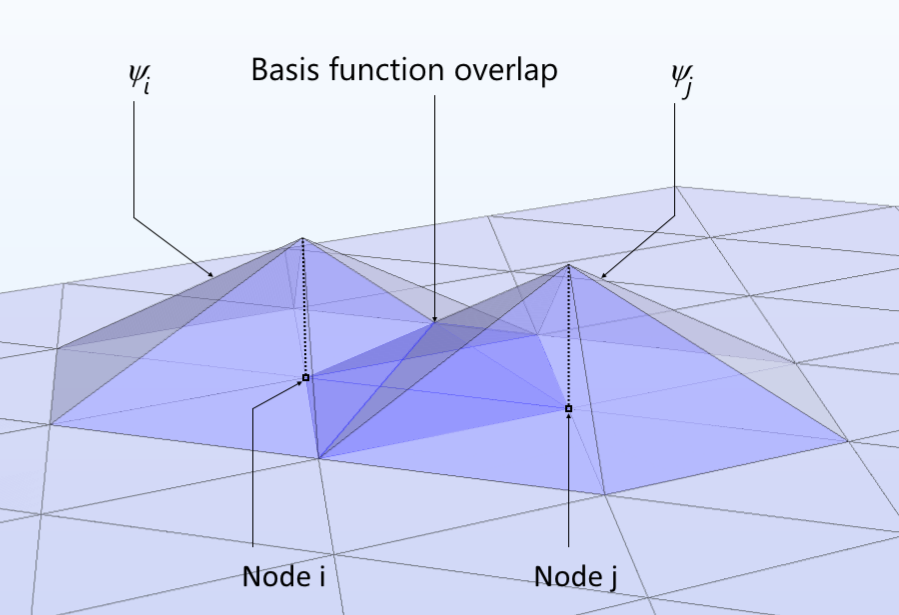
\includegraphics[width = 0.54\textwidth]{papers/fem/images/2d_basisfkt.png} \label{fem:nd:abb:basisfkt}}
    \caption{Ilustrationen von diskretisierten, zweidimensionalen Definitionsbereichen}
    \label{fem:nd:abb}
    \end{figure}
    
